\section[Руководство пользователя]{РУКОВОДСТВО ПОЛЬЗОВАТЕЛЯ}
\label{sec:user_manual}

Рассмотреть процесс установки программы (linux \& win).
Перечислить консольные аргументы.
% \subsection{Просмотр данных о наградах}
% \label{ssec:help_awards_list}

% Для того, чтобы перейти на страницу списка наград,
% необходимо нажать на пункт меню <<узнагароды>> (\textit{http://nagrady.by/award/list}),
% расположенный в правой верхней части страницы, 
% как показано на рисунке~\ref{fig:awards_link}.
% Ссылка на страницу списка наград отмечена красным цветом.

% \begin{figure}[h]
%   \centering
%   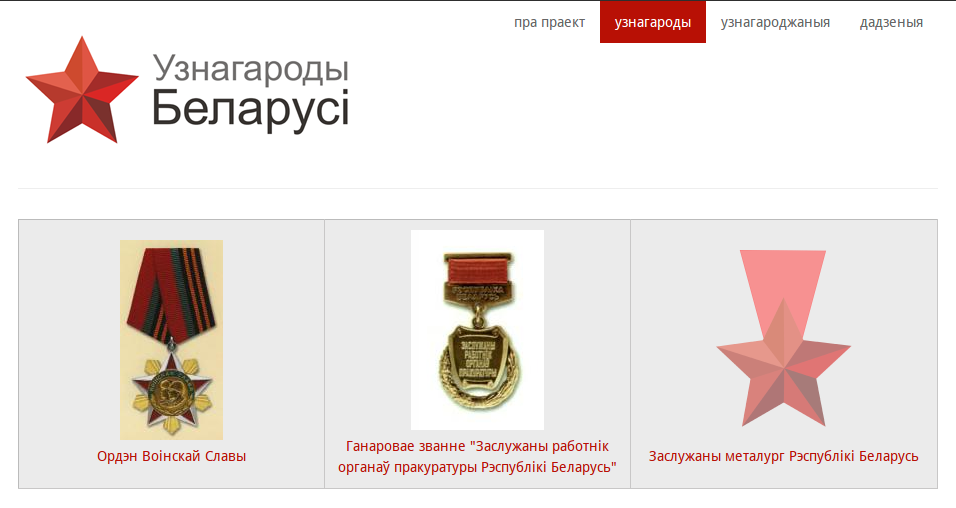
\includegraphics[width=160mm]{pic/help_awards_link.png}
%   \caption{Ссылка на список наград}
%   \label{fig:awards_link}
% \end{figure}

% Для того, чтобы просмотреть данные о конкретной награде,
% необходимо выполнить следующие действия:
% \begin{enumerate}
% \item Перейти на страницу списка наград.
% \item Выбрать награду, нажав на ссылку с названием нужной награды. 
% \end{enumerate}

% \subsection{Просмотр данных о награжденных}
% \label{ssec:help_awarded_list}

% Для того, чтобы перейти на страницу списка наград,
% необходимо нажать на пункт меню <<узнагароджаныя>> (\textit{http://nagrady.by/awarded/list}),
% расположенный в правой верхней части страницы, 
% как показано на рисунке~\ref{fig:awarded_link}.
% Ссылка на страницу списка награжденных отмечена красным цветом.

% \begin{figure}[h]
%   \centering
%   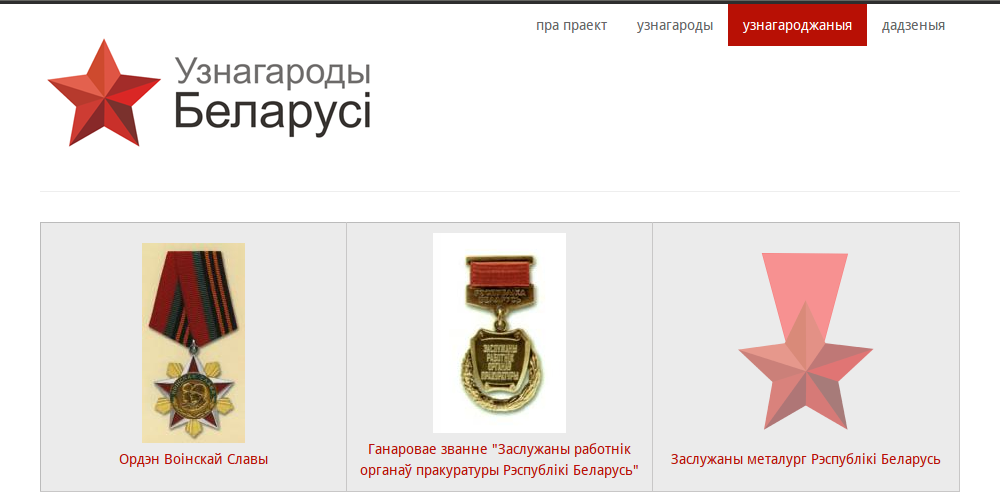
\includegraphics[width=160mm]{pic/help_awarded_link.png}
%   \caption{Ссылка на список награжденных}
%   \label{fig:awarded_link}
% \end{figure}

% Для того, чтобы просмотреть данные о конкретном факте награждения,
% необходимо выполнить следующие действия:
% \begin{enumerate}
% \item Перейти на страницу списка награжденных.
% \item Выбрать награду, нажав на ссылку с именем награжденного. 
% \end{enumerate}

% В результате вы будете находиться на странице с информацией о
% факте награждения, как показано на рисунке~\ref{fig:awarded_info}.

% \begin{figure}[h]
%   \centering
%   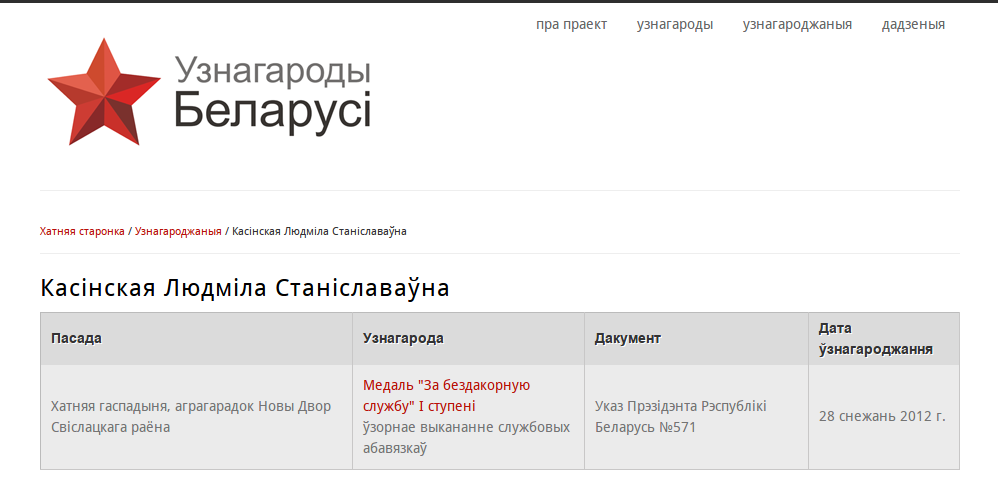
\includegraphics[width=160mm]{pic/help_awarded_info.png}
%   \caption{Страница с информацией о награжденном}
%   \label{fig:awarded_info}
% \end{figure}

% \subsection{Экспорт данных о фактах награждения}
% \label{ssec:help_export_awarded}

% Для того, чтобы экспортировать данные на локальный носитель,
% необходимо выполнить следующие шаги:
% \begin{enumerate}
% \item Перейти на страницу экспорта данных, 
%   нажав на пункт меню <<дадзеныя>> (\textit{http://nagrady.by/opendata}),
%   расположенный в правой верхней части страницы, 
%   как показано на рисунке~\ref{fig:opendata_link}.

% \begin{figure}[h]
%   \centering
%   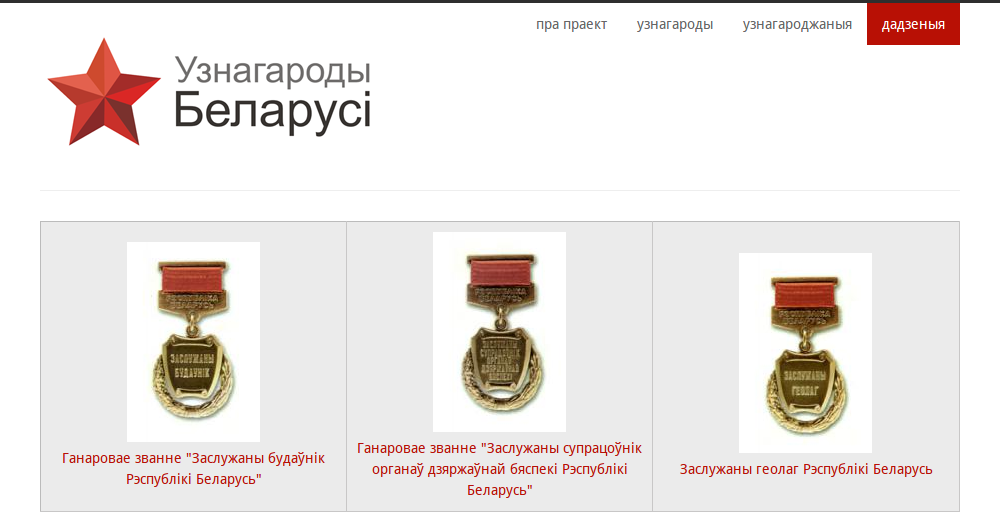
\includegraphics[width=160mm]{pic/help_opendata_link.png}
%   \caption{Ссылка на страницу экспорта данных о награжденных}
%   \label{fig:opendata_link}
% \end{figure}

% \item Воспользовавшись фильтрами по названию награды и дате награждения,
%   выбрать интересующий набор данных.
% \item Нажать кнопку \textit{<<CSV>>} или \textit{<<XML>>} в нижней части страницы, 
%   как показано на рисунке~\ref{fig:opendata_download} 
%   для экспорта в формате csv или xml соответственно.
% \end{enumerate}

% \begin{figure}[h]
%   \centering
%   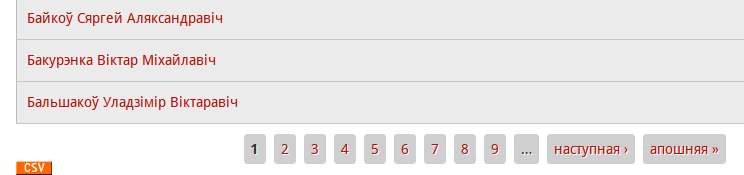
\includegraphics[width=150mm]{pic/help_opendata_download.png}
%   \caption{Кнопка экспорта данных о награжденных}
%   \label{fig:opendata_download}
% \end{figure}


% \subsection{Авторизация}
% \label{ssec:help_authorization}

% Для выполнения административных операций 
% (импорт и редатирование данных)
% пользователь должен войти в учетную запись администратора
% (пройти авторизацию).

% Для этого необходимо выполнить следующие действия:
% \begin{enumerate}
% \item Перейти по ссылке \textit{http://nagrady.by/user/login}.
% \item Ввести в поле \textit{<<Імя карыстальніка>>} имя учетной записи пользователя.
% \item Ввести в поле \textit{<<Пароль>>} пароль от учетной записи пользователя. 
% \item Нажать на кнопку \textit{<<Уваход у сістэму>>}.
% \end{enumerate}

% На рисунке~\ref{fig:login_page} изображена страница входа в учетную запись администратора.

% \begin{figure}[h]
%   \centering
%   {
%     \setlength{\fboxsep}{0pt}%
%     \setlength{\fboxrule}{1pt}%
%     \fbox{  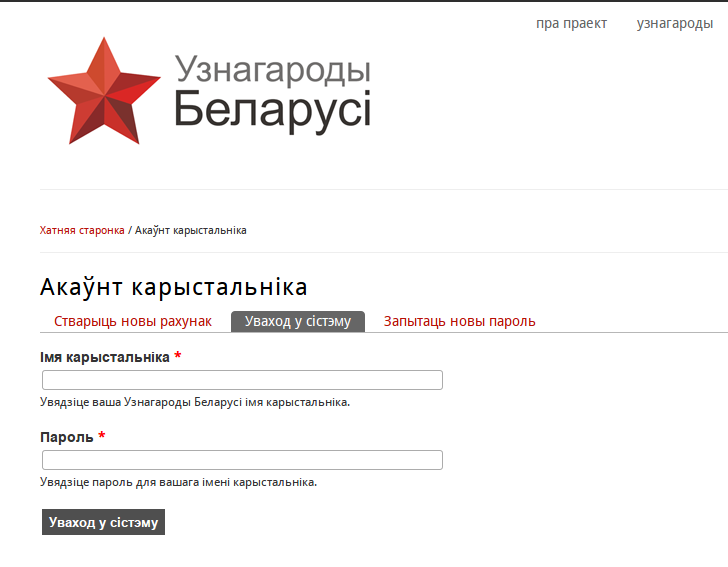
\includegraphics[width=150mm]{pic/login_page.png}}
%   }
%   \caption{Страница авторизации}
%   \label{fig:login_page}
% \end{figure}

% После успешной авторизации на каждой странице появится панель управления контентом сайта. 

% \subsection{Импорт данных о фактах награждения}
% \label{ssec:help_import_awarded}

% Для того, чтобы импортировать данные о наградах на сайт,
% необходимо сделать следующие шаги:

% \begin{enumerate}
% \item Пройти авторизацию на сайте в соответствии с подразделом~\ref{ssec:help_authorization}.
% \item После входа на сайт в качестве администратора перейти по ссылке <<Імпарт>>.
% \item На странице <<Узнагароды>>, показанной на рисунке~\ref{fig:import_page}
%   нажать на кнопку \textit{<<Choose File>>}.
% \item Выбрать файл с данными о фактах награждения в машиночитаемом формате.
% \item Опционально: выбрать разделитель, настроив поле \textit{<<Delimiter>>}.
% \item Опционально: можно отключить использование заголовков csv-файлов,
%    отметив поле \textit{<<No Headers>>}.
% \item Нажать на кнопку <<Імпарт>> для импорта содержимого файла в базу данных сервиса.
% \end{enumerate}

% \begin{figure}[h]
%   \centering
%   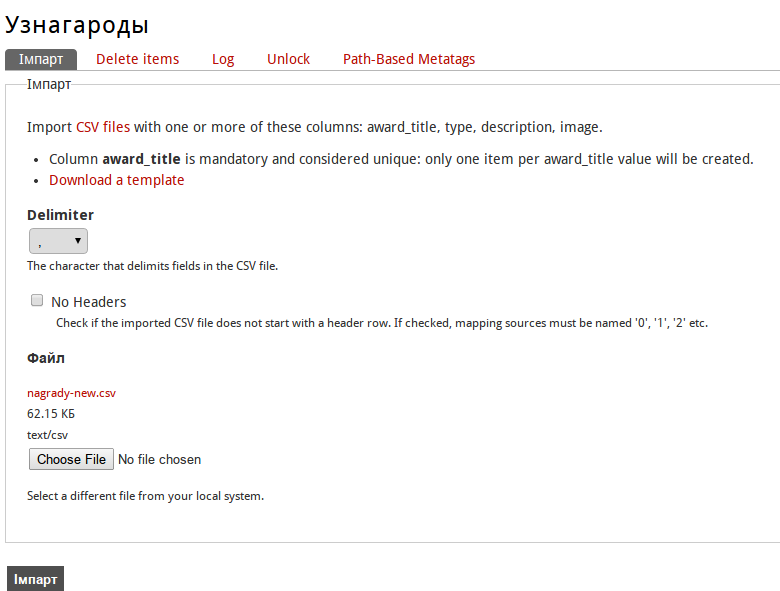
\includegraphics[width=150mm]{pic/import_page.png}
%   \caption{Страница импорта данных о фактах награждения}
%   \label{fig:import_page}
% \end{figure}

% \subsection{Редактирование данных о наградах}
% \label{ssec:help_edit_awards}

% Для того, чтобы отредактировать данные об определенной награде,
% необходимо сделать следующие шаги:

% \begin{enumerate}
% \item Пройти авторизацию на сайте в соответствии с подразделом~\ref{ssec:help_authorization}.
% \item После входа на сайт в качестве администратора
%    перейти по ссылке <<Кіраванне ўзнагародамі>>.
% \item На странице <<Кіраванне ўзнагародамі>> перейти по ссылке \textit{<<Edit>>},
%   расположенной в одной строке с названием требуемой награды.
% \item Отредактировать содержимое полей награды желаемым образом.
% \item Нажать на кнопку \textit{<<Save>>} для сохранения изменений.
% \end{enumerate}

% Интерфейс редактирования данных о наградах приведен
% на рисунке~\ref{fig:awards_edit_page}.

% \begin{figure}[h]
%   \centering
%   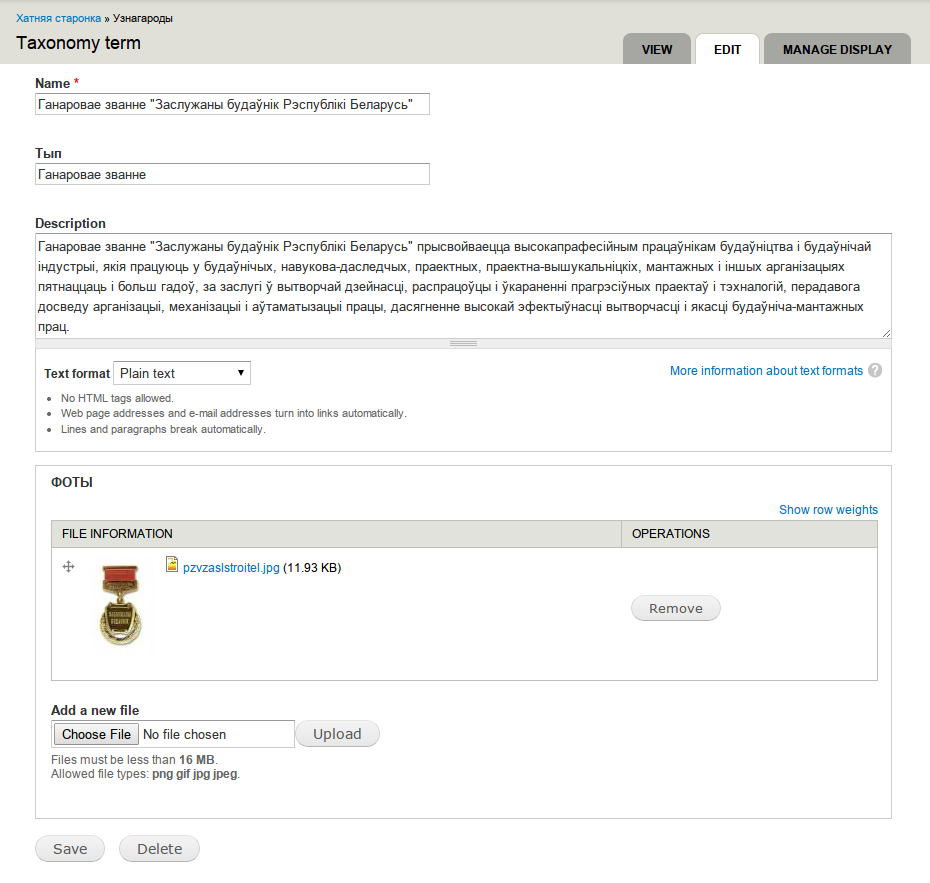
\includegraphics[width=150mm]{pic/awards_edit_page.png}
%   \caption{Интерфейс редактирования данных о награде}
%   \label{fig:awards_edit_page}
% \end{figure}


% \subsection{Редактирование данных о фактах награждения}
% \label{ssec:help_edit_awarded}

% Для того, чтобы отредактировать данные о факте награждения,
% необходимо сделать следующие шаги:

% \begin{enumerate}
% \item Пройти авторизацию на сайте в соответствии с подразделом~\ref{ssec:help_authorization}.
% \item После входа на сайт в качестве администратора
%    перейти по ссылке <<Кіраванне ўзнагароджанымі>>.
% \item На странице \textit{<<Content>>} перейти по ссылке \textit{<<Edit>>},
%   расположенной в одной строке с именем требуемого награжденного.
% \item Отредактировать содержимое полей награды желаемым образом.
% \item Нажать на кнопку \textit{<<Save>>} для сохранения изменений.
% \end{enumerate}

% Интерфейс редактирования данных о фактах награждения приведен 
% на рисунке~\ref{fig:awarded_edit_page}.

% \begin{figure}[h]
%   \centering
%   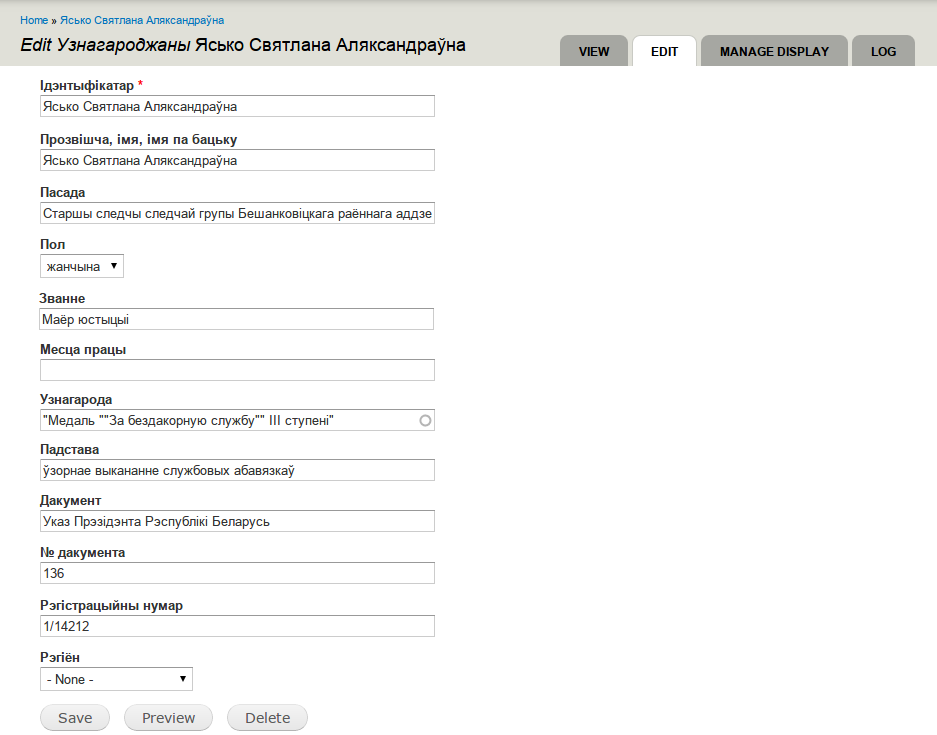
\includegraphics[width=160mm]{pic/awarded_edit_page.png}
%   \caption{Интерфейс редактирования данных о награжденном}
%   \label{fig:awarded_edit_page}
% \end{figure}
